% compile this on sharelatex.com
% !TEX program = pdflatex

\documentclass{scrartcl}
\usepackage[utf8]{inputenc}
\usepackage{graphicx}
\graphicspath{ {img/} }

\title{Submission Sheet 1}
\author{Danny Heinrich \and Matthias Kasperidus \and Leonard Kleinhans}
\date{29. October 2014}



\usepackage{amsmath}

\newcommand*\colvec[2]{
        \begin{pmatrix} #1 \\ #2 \end{pmatrix}
}

\begin{document}
\maketitle

\section{Exercise 1.1: McCulloch-Pitts Neural Net}
\item a) A two layered McCulloch-Pitts Neural Net is sufficient to model the given boolean function $f(x) = \bar x_1 \bar x_2 \bar x_3 \vee  x_1 x_2 \vee x_2 x_3 $ . Each conjunction is modelled by a neuron, which only fires if all three
inputs are active. The disjunction neuron fires as soon as one conjunction neuron fires. See Attachment 1

\item b) As seen in a) it is sufficient to use as two layered McCulloch-Pitts Neural Net to model the given boolean function g(x). 
The $\wedge$ binds stronger than the $\vee$ and therefore $g(x)$ is equivalent to $g(x) = x_1 x_2_x_3 \vee  x_1 x_2 \bar x_4\vee x_1 x_4 \bar x_2 $. See Attachment 2

\section{Exercise 1.2: Perceptron Classifier}

Apparently the given quadrangle is convex. So one can calculate the weight vectors $\vec{w_1},\vec{w_2},\vec{w_3},\vec{w_4}$ by deriving the four hyper planes.
It is easy to get the hyperplanes in the form $\vec{x} = \vec{p} + r \vec{q}$ with $\vec{x},\vec{p},\vec{q} \in R^2 ~r \in R$. This form is equivalent to the normalform $(\vec{x}-\vec{p})~\vec{n} = 0$ with normal vector $\vec{n}$, which can also be written as $\vec{x} ~ \vec{n} = \vec{p} ~ \vec{n}$ and is almost what we want. See Attachment 3 for the Quadrangle and Attachment 4 for the constructed net.\\
We now will calculate the four hyperplanes $H_{ab}$, $H_{bc}$, $H_{cd}$ and $H_{da}$ : \\
\begin{align*}
H_{ab}&: \vec{x} = \vec{a} + r (\vec{b}-\vec{a}) = \colvec{1}{1} + r \left(\colvec{2}{-2} - \colvec{1}{1}\right) = \colvec{1}{1} + r \colvec{-1}{-3} \\
\Leftrightarrow H_{ab}&: 3x_1 + x_2 = 4 \text{~with~} \vec{n} = \vec{w_1} = \colvec{3}{1} \\
H_{bc}&: \vec{x} = \vec{b} + r (\vec{c}-\vec{b}) = \colvec{2}{-2} + r \left(\colvec{0}{-1} - \colvec{2}{-2}\right) = \colvec{0}{-1} + r \colvec{-2}{1} \\
\Leftrightarrow H_{bc}&: (-1) x_1 + (-2) x_2 = 2 \text{~with~} \vec{n} = \vec{w_2} = \colvec{-1}{-2}\\
H_{cd}&: \vec{x} = \vec{c} + r (\vec{d}-\vec{c}) = \colvec{-1}{1} + r \left(\colvec{0}{-1} - \colvec{-1}{1}\right) = \colvec{-1}{1} + r \colvec{-1}{-2} \\
\Leftrightarrow H_{cd}&: 2 x_1 + (-1) x_2 = -3 \text{~with~} \vec{n} = \vec{w_3} = \colvec{2}{-1}\\
H_{da}&: \vec{x} = \vec{d} + r (\vec{a}-\vec{d}) = \colvec{-1}{1} + r \left(\colvec{1}{1} - \colvec{-1}{1}\right) = \colvec{-1}{1} + r \colvec{2}{0} \\
\Leftrightarrow H_{da}&: 2 x_2 = 2 \text{~with~} \vec{n} = \vec{w_4} = \colvec{0}{2}\\
\end{align*}

Because $(0,0)$ is inside the qudrangle, we can use that to get the inequalities:
\begin{align*}
3 x_1 + x_2 &\le 4 \\
-1 x_1 + -2 x_2 &\le 2 \\
2 x_1 + -1 x_2 &\ge 2 \\
2 x_2 &\le 2 \\
\end{align*}

\section{Exercise 1.3: Perceptron Learning}

As on can see in Figures 1 to 3 the perceptron learning algorithm correctly classifies only the third data set displayed in Figure 3. 
It shows that a singe layer perceptron learning algorithm can not classify every set correctly in such way that the algorithm terminates for given condition that every example must be classified correctly.
In fig. 3 one can see that precision and recall are close to 1 meaning that nearly all examples are classified correctly. Only a few false classified examples remain. This leads to the conclusion that the seperating hyperplane for the whole set can not be constructed.
A small error remains in every iteration of the algorithm. In figure 2 the precision rate drops drastically compared to figure 1 and 3. which induces a greater error. Finally the algorithm managed to determinate a weight vector to seperate the whole data set.
Since every example is correctly classified there are no more errors and thus precision and recall converge to 1.

To run the code first import the function with R-Studio by using the source() function or running the code inside R-Studio. 
After the function has been imported correctly it can be called in the R console taking 2 parameters. Perceptron(path,maxInit)
One possible approach would be : 
\item source("path/to/source/code/name.R)
\item Perceptron("path/to/data/set1.txt",maxIterations) with maxIterations taking positive integers, respresenting the maximum iterations.

\begin{figure}[ht]
\begin{center}
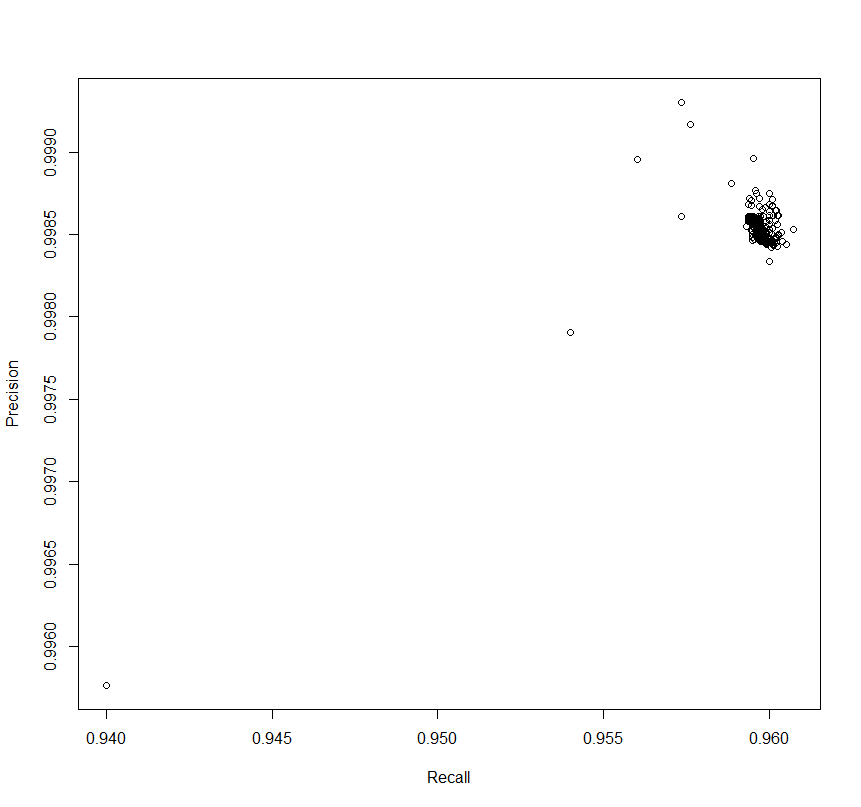
\includegraphics[scale=0.3]{PerceptronSet1.png}
\end{center}
\caption{Precision Recall Curve of Set 1.}
\label{Img:PrecisionRecallS1}
\end{figure}

\begin{figure}[ht]
\begin{center}
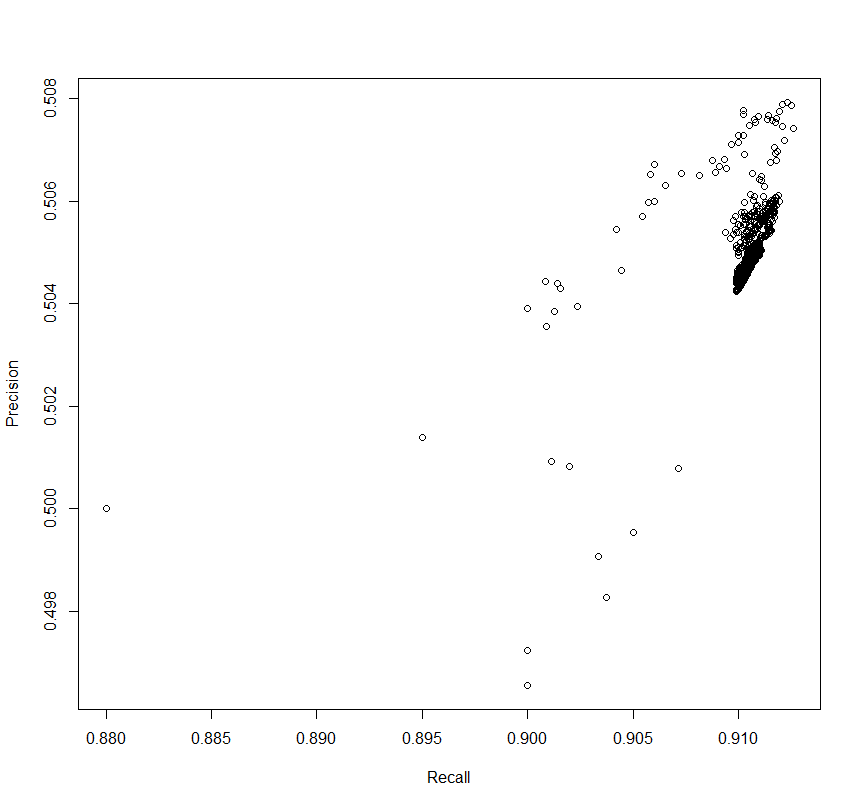
\includegraphics[scale=0.3]{PerceptronSet2.png}
\end{center}
\caption{Precision Recall Curve of Set 2.}
\label{Img:PrecisionRecallS1}
\end{figure}

\begin{figure}[ht]
\begin{center}
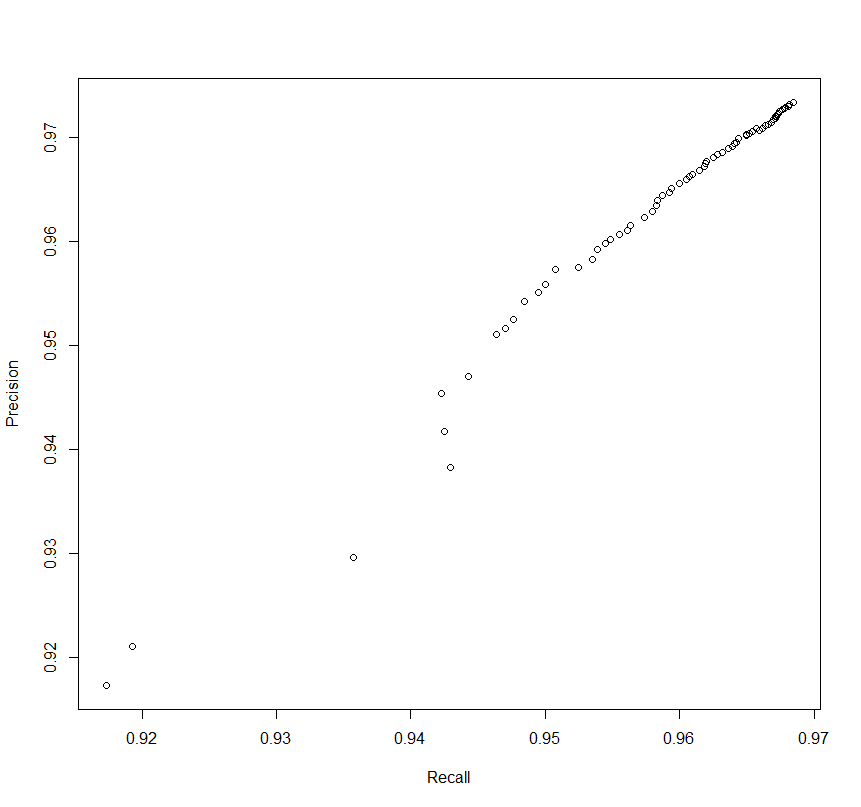
\includegraphics[scale=0.3]{PerceptronSet3.png}
\end{center}
\caption{Precision Recall Curve of Set 3.}
\label{Img:PrecisionRecallS1}
\end{figure}

\clearpage{}

\section{Exercise 1.4: Classification into more than two classes}
\begin{enumeration}
\item One option could be, to train for $N$ classes $n$ ANN's: Every ANN classifies if the input is in class $n \in N$ or not. Basically one would iterate over $\mathcal P \left({N}\right)$ in such way that $X \in \mathcal P \left({N}\right)$ contains all and only all classes which were correctly classified for a given input. Furthermore one would test if there is more than one set meeting this condition. The algorithm would return the set with the most classes in it.

\item Another possibility is to use two layered Perceptron classifiers to classify the input regarding a tuple of classes. After finding the correct class the algorithm would then take that class as another input and tuple it with a class, which has not been used yet.
As soon as all classes are processed by the algorithm the last correct class would be the one where the input would be most likely in.
\end{enumeration}

\item Another option are $2^n$ classifiers, one for every pair of classes. The algorithm would then return every class out of the tuple in which the input lies. The union over all returned classes would then suffice for a correct classification.

\end{enumeration}


\end{document}
